
\documentclass[12pt]{article}

\usepackage{amssymb, amsmath, amsfonts, bm, graphicx, geometry}
\usepackage{tabularx, booktabs, float, enumitem, multicol, mathtools}
\usepackage{parskip}
\usepackage{siunitx}
\usepackage[hidelinks]{hyperref}
\usepackage{soul}
\usepackage{mathrsfs}
\usepackage{fancyhdr}
\usepackage[most]{tcolorbox}

\geometry{margin=1in}

% List formatting
\setlist[itemize,1]{label=$\bullet$}
\setlist[itemize,2]{label=--}
\setlist[itemize,3]{label=$\circ$}
\setlist[itemize,4]{label=$\cdot$}

% US customary units
\DeclareSIUnit{\inch}{in}
\DeclareSIUnit{\foot}{ft}
\DeclareSIUnit{\yard}{yd}
\DeclareSIUnit{\mile}{mi}

\DeclareSIUnit{\slug}{slug}
\DeclareSIUnit{\lbm}{lbm}
\DeclareSIUnit{\lbf}{lbf}

\DeclareSIUnit{\psi}{psi}
\DeclareSIUnit{\psf}{psf}

\DeclareSIUnit{\gallon}{gal}
\DeclareSIUnit{\quart}{qt}
\DeclareSIUnit{\fahrenheit}{F}
\DeclareSIUnit{\rankine}{R}

\sisetup{
    per-mode = fraction
}

% Uppercase Volume with thicker, higher line
\newcommand{\vol}{\mathord{\text{\ooalign{\hidewidth $V$\hidewidth\cr\kern-0.5pt\raisebox{0.8ex}{\rule[0pt]{1em}{0.5pt}}}}}}

% Lowercase Volume with built-in shifts
\newcommand{\svol}{%
  \mathord{\text{\ooalign{%
    \hfil$v$\hfil\cr
    \hfil\rule[0.6ex]{0.8em}{0.5pt}\hfil
  }}}%
}

% Example box
\newtcolorbox{examplebox}[1][Example]{
    enhanced,
    breakable,
    colback=white,
    colframe=black!30,
    boxrule=0.4pt,
    arc=0pt,
    left=7pt, right=7pt,
    top=5pt, bottom=5pt,
    before upper={\textbf{Example: #1}\par\smallskip}
}

% Side note box
\newtcolorbox{notebox}[1][Side Note]{
    enhanced,
    breakable,
    colback=black!2,
    colframe=black!20,
    boxrule=0.3pt,
    arc=0pt,
    left=7pt, right=7pt,
    top=5pt, bottom=5pt,
    before upper={\textit{Side Note:} \textbf{#1}\par\smallskip}
}

% Header and Footer Setup
\pagestyle{fancy}
\fancyhf{}
\lhead{ESC 340M -- Fall 2026}
\rhead{Midterm 2 Practice}
\cfoot{\thepage}
\setlength{\headheight}{15pt}

% Title
\title{
    \textbf{ESC 340M: Fluid Mechanics}\\[0.5ex]
    \Large Midterm 2 Practice Problems
}
\author{Zeshui Song}
\date{Fall 2026}


\begin{document}
\maketitle
\vspace{-1em}
\subsection*{Problems 1--3: Fountain and Bob}
SupaDop, a trendy, youth-oriented shampoo brand, is getting ready to market RubyGlasz, a transparent red shampoo named after a popular vocal performer who inspired it. The marketing campaign will include a fountain of transparent red liquid that looks like red glass. The liquid stream will levitate an axisymmetric bob, which will neatly part the stream into an axisymmetric liquid sheet leaving the bob surface at an angle $\theta$ off the fountain ($z$) axis.
\begin{center}
    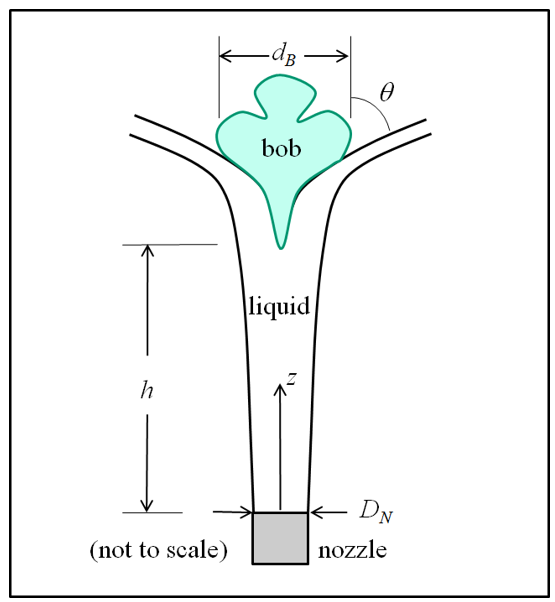
\includegraphics[width=0.5\textwidth]{prob1.png}
\end{center}
Gravity makes the liquid velocity decrease with distance above the fountain nozzle, $z$. The nozzle is designed so that the velocity profile exiting the nozzle is uniform, and the velocity remains uniform in the liquid stream below the bob. The equation for velocity is given by
\[
V(z)=\sqrt{V_N^2-2gz}. \tag{1}
\]
where $V_N$ is the liquid speed exiting the nozzle, $z$ is the height above the nozzle, and $g$ is the gravitational constant. Equation (1) is valid until the liquid reaches the bob tip. Assume the fountain operates at steady state. Furthermore, you can assume that the speed of the water coming off the bob is the same as the speed of the water in the stream when it first encounters the bob.

\subsection*{Problem 1 (25 pts.)}
Derive an expression for the liquid stream diameter as a function of distance $z$ above the nozzle, and other key problem parameters.

\paragraph{Solution}\mbox{}\\
Since the fluid velocity decreases with height (gravity slows it down), the cross-sectional area of the stream must increase to conserve mass. Therefore, I can use the conservation of mass with Reynolds transport theorem to derive the expression for the stream diameter as a function of height $z$.\\\\
Defining the fixed control volume:
\begin{center}
    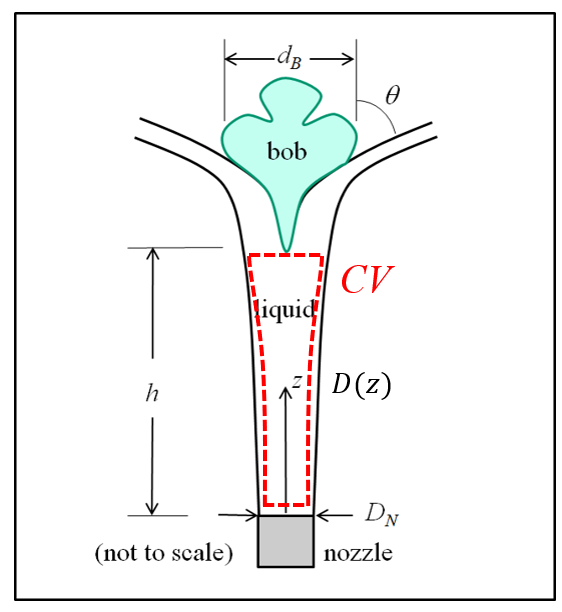
\includegraphics[width=0.35\textwidth]{prob1-1.png}
\end{center}
Reynolds transport theorem:
\[\frac{DM_{\text{sys}}}{Dt} = 0 = \frac{\partial}{\partial t}\int_{C\vol} \rho \, dV + \int_{CS} \rho \vec{V}_{\text{rel}} \cdot \hat{n} \, dA\]
Assume:
\begin{itemize}
    \item Steady state: fixed control volume with no change in density over time
    \[\frac{\partial}{\partial t}\int_{C\vol} \rho \, dV = 0\]
    \item Incompressible flow: $\rho$ is constant
    \item Uniform velocity across the stream cross-section: can be taken outside of the surface integrals
    \item No flow through the control volume sides, only 1 inlet and 1 outlet
    \item Fixed control volume: $\vec{V}_{\text{rel}} = \vec{V}$
\end{itemize}
Therefore:
\[-\rho V(0) \left(\frac{\pi D_N^2}{4}\right) +\rho V(z) \left(\frac{\pi D(z)^2}{4}\right) = 0\]
Solving for $D(z)$:
\[\boxed{
\begin{aligned}
D(z)&=D_N\sqrt{\frac{V(0)}{V(z)}}\\
&=D_N\left(1-\frac{2gz}{V_N^2}\right)^{-1/4}
\end{aligned}}
\]
\subsection*{Problem 2 (25 pts.)}
The artist who created the fountain wants you to control the bob height $h$ while they vary the fountain nozzle diameter $D_N$, bob diameter $d_B$ and mass $M_B$, and parting angle $\theta$ in the design. Derive an expression (design equation) for the steady state bob height, $h$, as a function of $V_N$, the bob parameters, and the fluid properties. You may ignore the effects of viscosity in your model.
\paragraph{Solution}\mbox{}\\
Here, we can use the conservation of linear momentum to determine the forces acting on the bob in terms of the flow velocity (which is a function of height $h$).\\\\
Defining the control volume around the bob:
\begin{center}
    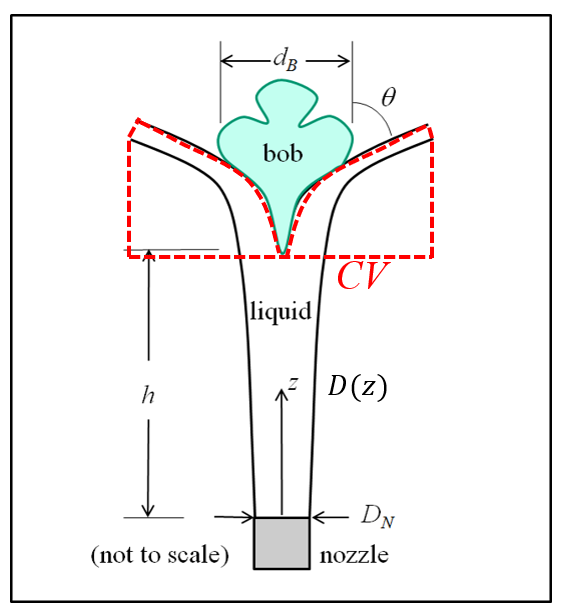
\includegraphics[width=0.35\textwidth]{prob1-2.png}
\end{center}
Reynolds transport theorem:
\[\frac{D\vec{P}_\text{sys}}{Dt} = \sum \vec{F}_{\text{ext}} = \frac{\partial}{\partial t}\int_{C\vol} \rho \vec{V} \, d\vol + \int_{CS} \rho \vec{V} (\vec{V}_{\text{rel}}\cdot \hat{n}) \, dA\]
\newpage
Assume:
\begin{itemize}
    \item Steady state: fixed control volume with no change in momentum over time
    \[\frac{\partial}{\partial t}\int_{C\vol} \rho \vec{V} \, d\vol = 0\]
    \item Incompressible flow: $\rho$ is constant
    \item Uniform velocity across the stream
    \item Same fluid velocity at the inlet and outlet of the control volume
    \item Fixed control volume: $\vec{V}_{\text{rel}} = \vec{V}$
    \item Considering only the vertical force balance to find the operating height of the bob
\end{itemize}
Also assuming negligible fluid weight:
\begin{align*}
F_{\text{bob on fluid, z}} =& \rho(V(h))(-V(h))\left(\frac{\pi D(h)^2}{4}\right)+(V(h)\cos\theta)(V(h))A_{\text{outlet}}\\
=& -\rho V(h)^2\left(\frac{\pi D(h)^2}{4}\right)+\rho V(h)^2\cos\theta A_{\text{outlet}}
\end{align*}
Using continuity to relate the outlet area to the inlet area:
\[
V(h)A_{\text{in}}=V(h)A_{\text{out}}\quad\implies\quad A_{\text{out}}=A_{\text{in}}=\frac{\pi D(h)^2}{4}
\]
Therefore,
\[
\boxed{F_{\text{bob on fluid},z}=\rho V(h)^2\frac{\pi D(h)^2}{4}(\cos\theta-1)}
\]
Now considering the forces acting on the bob in the vertical direction:
\[F_{\text{fluid on bob},z} = -F_{\text{bob on fluid},z}\]
\[\sum F_\text{ext on bob, z} = F_{\text{fluid on bob},z} - M_B g = 0\]
At equilibrium:
\[-\rho V(h)^2\frac{\pi D(h)^2}{4}(\cos\theta-1) - M_B g = 0\]
\[
\begin{aligned}
\rho V(h)^2\frac{\pi D(h)^2}{4}(1-\cos\theta)-M_Bg&=0\\
\rho V(h)V_N\frac{\pi D_N^2}{4}(1-\cos\theta)&=M_Bg
\qquad \text{(from prob 1)}\\
V(h)&=\frac{4M_Bg}{\rho\pi D_N^2V_N(1-\cos\theta)}\\
V_N^2-2gh&=\left(\frac{4M_Bg}{\rho\pi D_N^2V_N(1-\cos\theta)}\right)^2
\end{aligned}
\]
\[
\boxed{
h=\frac{1}{2g}\left[
V_N^2-
\left(
\frac{4M_Bg}{\rho\pi D_N^2V_N(1-\cos\theta)}
\right)^2
\right]
}
\]


\subsection*{Problem 3 (10 pts.)}
Calculate the steady state bob height $h$ for the tabulated parameter values.

\begin{center}
\begin{tabular}{lll}
\toprule
Parameter & Value & Units \\
\midrule
$D_N$ & 3.5 & cm \\
$V_N$ & 6 & m/s \\
$\rho$ & 1200 & kg/m$^3$ \\
$M_B$ & 1.3 & kg \\
$d_B$ & 8 & cm \\
$\theta$ & 60 & degrees \\
\bottomrule
\end{tabular}
\end{center}

\paragraph{Solution}\mbox{}
\[
\begin{aligned}
h&=\frac{1}{2g}\left[
V_N^2-\left(
\frac{4M_Bg}{\rho\pi D_N^2V_N(1-\cos\theta)}
\right)^2\right]\\
&=\frac{1}{2(\SI{9.81}{\meter\per\second\squared})}
\left[
(\SI{6}{\meter\per\second})^2-
\left(
\frac{
4(\SI{1.3}{\kilogram})(\SI{9.81}{\meter\per\second\squared})
}{
(\SI{1200}{\kilogram\per\meter\cubed})
\pi\left(\SI{3.5}{\centi\meter}\cdot
\frac{\SI{1}{\meter}}{\SI{100}{\centi\meter}}\right)^2
(\SI{6}{\meter\per\second})(1-\cos60^\circ)
}
\right)^2
\right]\\
&=\boxed{\SI{1.144}{\meter}}
\end{aligned}
\]



\subsection*{Problem 4 (20 pts.)}
SupaDop RubyGlasz shampoo is rather viscous and has some gel-like qualities, \hl{and it doesn't flow if the shear stress is below a yield stress}. Furthermore, the artist creating the fountain wants you to look into running the shampoo in the fountain (you would prefer to use water), so both you and the packaging department need to get a viscosity vs. shear rate curve for the shampoo. To make some initial measurements prior to finding the right viscometer, you set up a system like the one sketched in the figure, with a plate of mass $M$, length $L$, and width $W$, sliding over a layer of shampoo of height $h$, driven by a hand-held spring balance. While holding the balance force approximately constant at $F=2\,\mathrm{N}$, you take a cell phone movie and measure the time $\Delta t$ required to slide the plate one plate length, $L$. Estimate the shampoo viscosity and shear rate from this crude experiment. Parameter values and measurements are listed in the table.

\begin{center}
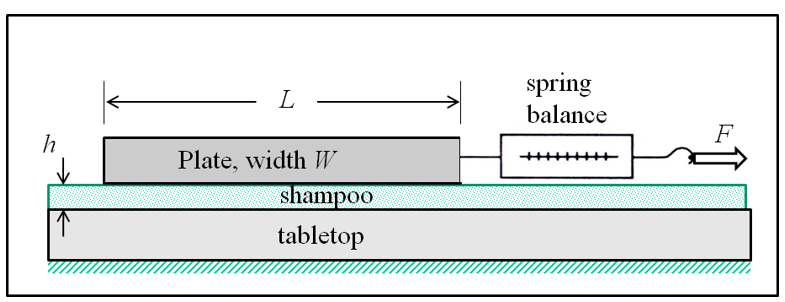
\includegraphics[width=0.6\textwidth]{prob4.png}
\end{center}

\begin{center}
\begin{tabular}{lll}
\toprule
Parameter & Value & Units \\
\midrule
$h$ & 1 & mm \\
$L$ & 0.2 & m \\
$W$ & 0.1 & m \\
$M$ & 0.126 & kg \\
$\Delta t$ & 0.87 & s \\
$F$ & 2 & N \\
\bottomrule
\end{tabular}
\end{center}

\paragraph{Solution}\mbox{}\\
Viscosity is relates to shear stress by the equation:
\[\tau = \mu \dot{\gamma} = \mu \frac{du}{dy}\]
Where $du/dy$ is the derivative of the velocity gradient. Assuming a linear velocity profile, we can approximate the shear rate as:
\[\dot{\gamma} = \frac{du}{dy} \approx \frac{V}{h}\]
Where $V$ is the velocity of the plate and $h$ is the height of the shampoo layer.\\\\
$V$ is approximated by:
\[V\approx \frac{L}{\Delta t}\]
Therefore:
\[\tau \approx \mu \frac{L}{h \Delta t}\]
Assuming the plate is sliding at a constant velocity, the average shear stress is:
\[\sum F_x = 0\quad \implies \quad F=\tau LW\]
Putting it all together, viscosity and shear rate can be estimated as:
\[\dot{\gamma} \approx \frac{L}{h \Delta t}\]
\[\mu \approx \frac{\tau}{\dot{\gamma}} = \frac{F}{LW} \cdot \frac{h \Delta t}{L} = \frac{F h \Delta t}{L^2 W}\]
Subbing in values:

\[
\begin{aligned}
\dot{\gamma}
&\approx \frac{L}{h\Delta t}\\
&=\frac{\SI{0.2}{\meter}}
{\left(\SI{1}{\milli\meter}\cdot\frac{\SI{1}{\meter}}{\SI{1000}{\milli\meter}}\right)
(\SI{0.87}{\second})}\\
&=\boxed{\SI{229.89}{\per\second}}
\end{aligned}
\]

\[
\begin{aligned}
\mu
&\approx \frac{Fh\Delta t}{L^2W}\\
&=\frac{(\SI{2}{\newton})
\left(\SI{1}{\milli\meter}\cdot\frac{\SI{1}{\meter}}{\SI{1000}{\milli\meter}}\right)
(\SI{0.87}{\second})}
{(\SI{0.2}{\meter})^2(\SI{0.1}{\meter})}\\
&=\boxed{\SI{0.435}{\pascal\second}}
\end{aligned}
\]

\subsection*{Problem 4: Extra Credit (6 pts.)}
An inventive member of the team suggests that it might be better to drive the shampoo between two fixed parallel plates, using a compressed air source with a regulator, and measuring the flow rate. Explain in detail how this might work for a Newtonian liquid, and explain why for the shampoo it would be rather complicated.

\paragraph{Solution}\mbox{}\\
\textit{review this}\\
Model pressure-driven flow between two fixed parallel plates using the Navier-Stokes equations.

For an incompressible Newtonian fluid:
\[
\rho\left(\frac{\partial\vec V}{\partial t}
+(\vec V\cdot\nabla)\vec V\right)
=-\nabla p+\rho\vec g+\mu\nabla^2\vec V
\]

Expanding the $x$-component:
\[
\rho\left(
\frac{\partial u}{\partial t}
+u\frac{\partial u}{\partial x}
+v\frac{\partial u}{\partial y}
+w\frac{\partial u}{\partial z}
\right)
=-\frac{\partial p}{\partial x}
+\rho g_x
+\mu\left(
\frac{\partial^2u}{\partial x^2}
+\frac{\partial^2u}{\partial y^2}
+\frac{\partial^2u}{\partial z^2}
\right)
\]

Assume:
\begin{itemize}
    \item Steady flow: $\partial/\partial t=0$.
    \item Fully developed flow: $\partial u/\partial x=0$.
    \item Unidirectional flow: $\vec V=u(y)\hat i$, so $v=w=0$.
    \item Wide plates: $\partial u/\partial z=0$.
    \item Horizontal plates: $g_x=0$.
\end{itemize}

Therefore, the $x$-momentum equation reduces to:
\[
\boxed{0=-\frac{dp}{dx}+\mu\frac{d^2u}{dy^2}}
\]

Integrate twice and apply the no-slip boundary conditions
$u(0)=u(h)=0$ to obtain the velocity profile. Then integrate
over the cross-sectional area to find $Q$ and solve for $\mu$.\\\\
However, this method would be complicated for the shampoo because it is a non-Newtonian fluid with a yield stress and therefore the viscosity would not be constant.


\subsection*{Problem 5 (20 pts.)}
RubyGlasz (the performing artist) decides that it would be fun to fill some red balloons with the shampoo and throw them into the audience during the launch party/concert. They will fill each balloon to a pressure of about $0.5\,\mathrm{psig}$. The artist wants you to think about and explain the shape of these shampoo (water) balloons.

\begin{center}
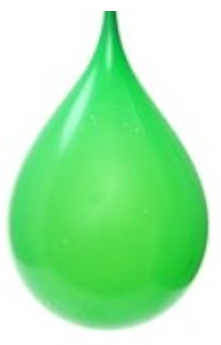
\includegraphics[width=0.15\textwidth]{prob5.png}
\end{center}

\begin{enumerate}
    \item[(a)] If the pressure is $0.5\,\mathrm{psig}$ at the top of the balloon, and it is completely filled with shampoo, what is the pressure distribution inside the balloon? (Make a sketch, and label minimum and maximum pressures.)
    \paragraph{Solution}\mbox{}\\
    This is just the hydrostatic pressure distribution with the minimum pressure at the top of the balloon and the maximum pressure at the bottom of the balloon. Pressure increases downwards and points normal to the interior of the balloon.
    \item[(b)] Estimate the maximum pressure if the height of the balloon is $30\,\mathrm{cm}$ and the shampoo density is $1200\,\mathrm{kg/m^3}$.
    \paragraph{Solution}\mbox{}\\
    Still hydrostatic pressure distribution.
    \item[(c)] Discuss how the pressure distribution affects the balloon's shape, compared to an air-filled balloon.
    \paragraph{Solution}\mbox{}\\
    Because pressure increases with depth, the lower portion of the balloon experiences a greater outward pressure difference than the upper portion.

Therefore, a shampoo-filled balloon tends to bulge more near the bottom, whereas an air-filled balloon has nearly uniform internal pressure because the hydrostatic pressure variation in air is much smaller. (Since the density of air is much lower than that of shampoo, the pressure difference from top to bottom in an air-filled balloon is negligible.)
\end{enumerate}

\subsection*{Problem 6: Extra Credit (5 pts.)}
Continuing from Problem 5, imagine putting a filled balloon on a glass table. Devise a method to use the diameter of the contact patch between the balloon and the table to estimate the pressure at the top of the balloon.

\paragraph{Solution}\mbox{}\\
For the balloon to be at rest on the table, the pressure at the bottom of the balloon must equal the weight of the balloon divided by the area of the contact patch. Therefore
\[
p_{\text{bottom}}-p_{\text{atm}}\approx\frac{Mg}{A_c}
\]
then we can relate the pressure at the bottom to the pressure at the top using hydrostatic pressure.

\subsection*{Problem 7: Extra Credit (5 pts.)}
Researching the shampoo balloon on the internet, I found confusing results for the air pressure in a party balloon. The first answer (in a box!) that I got from Google was that the pressure inside a balloon is 14.7 psi, and this was repeated several times. Discuss what is right (or useful) and what is wrong (or useless) with this answer.

\paragraph{Solution}\mbox{}\\
This all depends on gauge vs absolute pressure. Since the atmospheric pressure is about 14.7 psi, the absolute pressure inside a must be higher than that to keep it inflated. So its not very useful or correct to say that the pressure inside a balloon is 14.7 psi, because that is the atmospheric pressure. 

\subsection*{Problem 8: Extra Credit (5 pts.)}
Derive the expression for $V(z)$ in equation (1), listing all assumptions that are required.

\paragraph{Solution}\mbox{}\\
Using bernoulli's equation along a streamline from the nozzle to a point at height $z$:
\[
\frac{p}{\rho}+\frac{V^2}{2}+gz=\text{constant}
\]
At nozzle exit, $z=0$, $V=V_N$, and $p=p_\text{atm}$. At height $z$, $V=V(z)$ and $p=p_\text{atm}$ (free jet condion). Therefore:
\[
\frac{V_N^2}{2}=\frac{V(z)^2}{2}+gz
\]
\[
\boxed{V(z)=\sqrt{V_N^2-2gz}}
\]
\end{document}
